\documentclass[10pt,a4paper]{article}
\usepackage[utf8]{inputenc}
\usepackage[russian]{babel}
\usepackage[OT1]{fontenc}
\usepackage{amsmath}
\usepackage{amsfonts}
\usepackage{amssymb}
\usepackage{graphicx}
\usepackage{placeins}
\graphicspath{{lab4/},{lab5/},{lab6/},{lab7/}}


\author{Климов С.А., Назарова К.Е.}
\title{Отчет по лабораторным работам по дисциплине ТСС}
\date{2014}
\begin{document}
\maketitle
\pagebreak
\tableofcontents
\pagebreak
\section{Система верстки \TeX и расширения \LaTeX}
\subsection{Цель работы}
Изучение принципов верстки ТеХ, создание первого отчета
\subsection{Ход работы}
\paragraph{Изучение}
\begin{enumerate}
\item Создание минимального файла .tex в простом текстовом редакторе - преамбула, тело документа
\item Компиляция в командной строке - latex, xdvi, pdflatex
\item Оболочка TexMaker, Быстрый старт, быстрая сборка
\item Создание титульного листа, нескольких разделов, списка, несложной формулы
\end{enumerate}
\paragraph{Выполнение практического задания}
\begin{displaymath}
c^2 = a^2 + b^2
\end{displaymath}
\begin{equation}
c_1+c_2=b_0\frac{2*a}{\log2}
\sum_{i=0}^{\infty}\Theta
\end{equation}
\begin{equation}
b(k) = (-1)^k\frac{2}{N}\sum_{n=0}^{\frac{N}{2}-1}a(n)cos{\frac{\pi k(2n+1)}{N}}
\end{equation}
\begin{equation}
R_2=\frac{(|A|+1)/(\pi f_c C_1)}{b+\sqrt{b^2-4c(|A|+1)C_2/C_1}}
\end{equation}
\subsection{Выводы}
При выполнении данной работы мы ознакомились с ситемой верстки \TeX  и расширением \LaTeX. Были получены начальные навыки верстки документа, а также построения различного вида формул.
\subsection{Материалы}
\begin{enumerate}
\item Не очень краткое введение
\item Конспект-справочник
\item http://www.inp.nsk.su/~baldin/LaTeX/lurs.pdf
\item Математика в \LaTeX
\end{enumerate}
\subsection{Инструменты}
\begin{enumerate}
\item TeX для Windows ProText
\item TeXnicCenter
\item TeXmaker
\end{enumerate}
\section{Визуализация сигналов во временной и частотной области}
\subsection{Цель работы}
Познакомиться со средствами генерации сигналов и визуализации их спектров.
\subsection{Постановка задачи}
В командном окне MATLAB и в среде Simulink промоделировать чистый синусоидальный сигнал, а также синусоидальный сигнал с шумом. Получить их спектры.
\subsection{Справочные материалы}
В.С. Гутников Фильтрация измерительных сигналов пп.1-2, 11-12
\subsection{Ход работы}
В среде MATLAB вначале моделируем чистый синусоидальный сигнал по формуле:
\begin{displaymath}
A(t) = A_0sin(2\pi ft + f_0)
\end{displaymath}
Затем моделируем зашумленный сигнал по формуле:
\begin{displaymath}
A(t) = A_0sin(2\pi ft + f_0) + A_1 rand()
\end{displaymath}
Для выделения частот регулярных составляющих используем преобразование Фурье, которое реализовано встроенной в MATLAB функцией.
\paragraph{Код MATLAB}
\begin{flushleft}
f = 10;\\
x = 0:0.01:8*pi;\\
y = sin(2*pi*f*x+pi/2);\\
plot(x(1:200),y(1:200))\\
grid\\
figure\\
spectrum = fft(y,512);\\
norm\_spectrum = spectrum.*conj(spectrum)/512;\\
f=100*(0:511)/512;\\
plot(f, norm\_spectrum(1:512))\\
axis([0 max(f) 0 10])\\
grid\\
y\_noise = y + 0.6 * rand(size(x));\\
figure\\
plot(x(1:200),y\_noise(1:200));\\
grid\\
spectrum\_noise = fft(y\_noise,512);\\
noise\_spectrum = spectrum\_noise.*conj(spectrum\_noise)/512;\\
figure\\
plot(f, noise\_spectrum(1:512))\\
axis([0 max(f) 0 10])\\
grid\\
\end{flushleft}
\subsection{Результаты работы}
В результате получаем следующие графики временных и частотных характеристик для чистого и зашумленного синусоидального сигналов:

\begin{figure}[h]
\centering
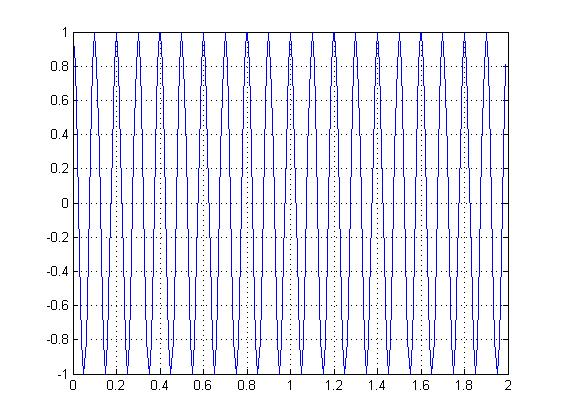
\includegraphics[width=10cm]{1.jpg} 
\caption{Временная характеристика чистого синусоидального сигнала} 
\label{fig.0} 
\end{figure}
\newpage
\begin{figure}[h]
\centering
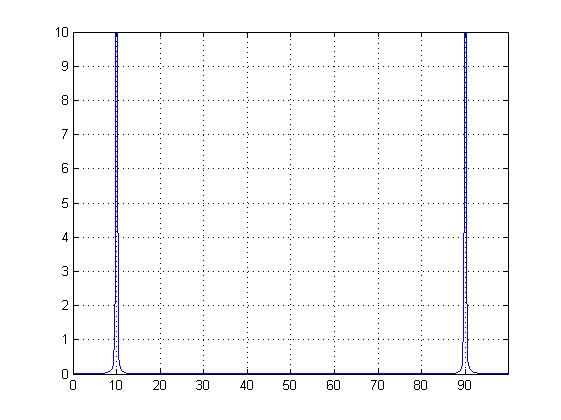
\includegraphics[width=10cm]{2.jpg} 
\caption{Частотная характеристика чистого синусоидального сигнала} 
\label{fig.1} 
\end{figure}
\begin{figure}[h]
\centering
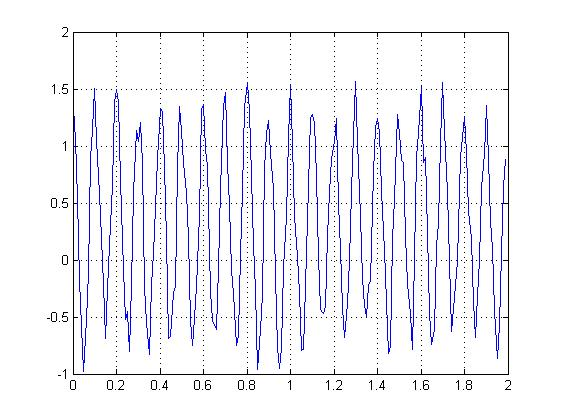
\includegraphics[width=10cm]{3.jpg} 
\caption{Временная характеристика зашумленного синусоидального сигнала} 
\label{fig.2} 
\end{figure}
\newpage
\begin{figure}[h]
\centering
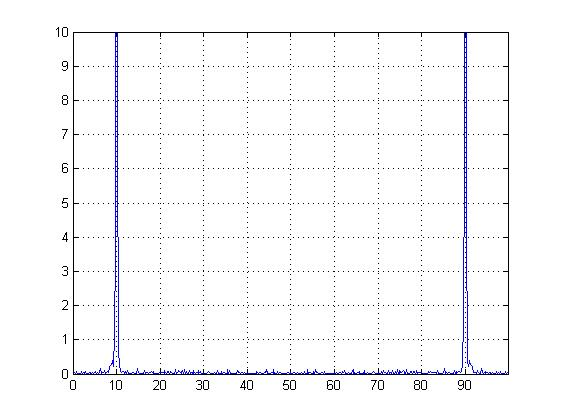
\includegraphics[width=10cm]{4.jpg} 
\caption{Частотная характеристика зашумленного синусоидального сигнала} 
\label{fig.3} 
\end{figure}

\subsection{Выводы}
\newpage
По результатам моделирования синусоидальных сигналов (чистого и с шумом) а также их полученных спектров можно сделать следующие выводы: умноженный на свое комплексное сопряженное спектр является нормированным, синус не бесконечен, спектр испытывает свертку с синком, повторение спектра происходит на частоте, кратной частоте дискретезации.

\newpage
\section{Спектры простых сигналов}
\subsection{Цель работы}
Получить представление о свойствах спектров.
\subsection{Постановка задачи}
В командном окне MATLAB и в среде Simulink промоделировать следующие тестовые сигналы:
\begin{itemize}
\item Полигармонический сигнал 
	\begin{equation}
	y(t) = \sum_{n=0}^{{N}-1}cos{(nt)}
	\end{equation}
\item Прямоугольный импульсный сигнал
	\begin{equation}
	y(t) = \prod(t, T_i)
	\end{equation}
\item Tреугольный импульсный сигнал
	\begin{equation}
	y(t) = \vartriangle(t, T_i)
	\end{equation}
\end{itemize}
и получить их спектры.
\subsection{Справочные материалы}
В.С. Гутников. Фильтрация измерительных сигналов пп.3-6, 13-14
\subsection{Ход работы}
Для моделирования заданных сигналов использовался приведенный код MATLAB:

\begin{flushleft}
t = 0:00.1:4*pi;\\
N = 100;\\
y = 0;\\

\% Полигармонический сигнал\\
y = sin(pi*t)+sin(2*pi*t)+sin(pi*0.3*t);\\
plot(t,y,'LineWidth',2)\\
grid\\

figure\\
spectrum = fft(y,512);\\
norm\_spectrum = spectrum.*conj(spectrum)/512;\\
f=100*(0:255)/512;\\
plot(f, norm\_spectrum(1:256),'LineWidth',2)\\
axis([0 max(f) 0 10])\\
grid\\

\% Прямоугольный сигнал\\
figure\\
y1 = square(t,50);\\
plot(t(1:100),y1(1:100),'LineWidth',2);\\
ylim([-2,2]);\\
grid\\

figure\\
spectrum = fft(y1,512);\\
norm\_spectrum = spectrum.*conj(spectrum)/512;\\
f1=100*(0:255)/512;\\
plot(f1, norm\_spectrum(1:256),'LineWidth',2)\\
axis([0 max(f1) 0 10])\\
grid\\

\% Треугольный сигнал\\
figure\\
y2 = conv(square(t,20),square(t,20));\\
plot(t(1:100),y2(1:100),'LineWidth',2);\\
grid\\

figure\\
spectrum = fft(y2,512);\\
norm\_spectrum = spectrum.*conj(spectrum)/512;\\
f2=100*(0:255)/512;\\
plot(f2, norm\_spectrum(1:256)/1000,'LineWidth',2)\\
axis([0 max(f2) 0 50])\\
grid\\
\end{flushleft}
\subsection{Результаты работы}
В результате были получены следующие сигналы и их спектры:


\begin{figure}[h]\centering
  \parbox[b]{0.49\textwidth}{\centering
    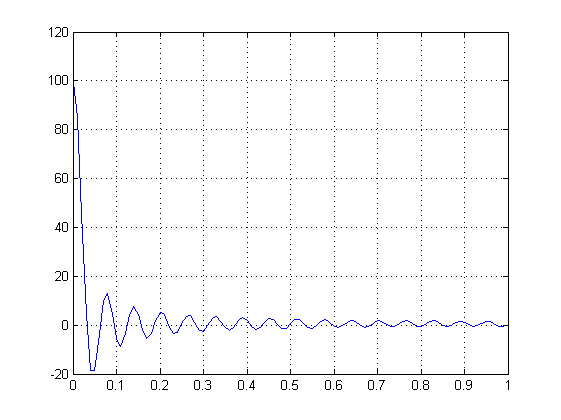
\includegraphics[width=6.5cm]{5_1} 
    \caption{Полигармонический сигнал}\label{fig.l5_1}}
  \hfil\hfil 
  \begin{minipage}[b]{0.49\textwidth}
	\centering
	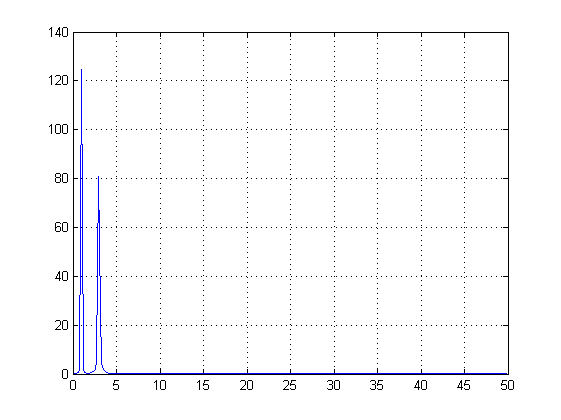
\includegraphics[width=6.5cm]{5_2}
	\caption{Спектр полигармонического сигнала}\label{fig.l5_2} 
  \end{minipage}
\end{figure}

\begin{figure}[h]\centering
  \parbox[b]{0.49\textwidth}{\centering
    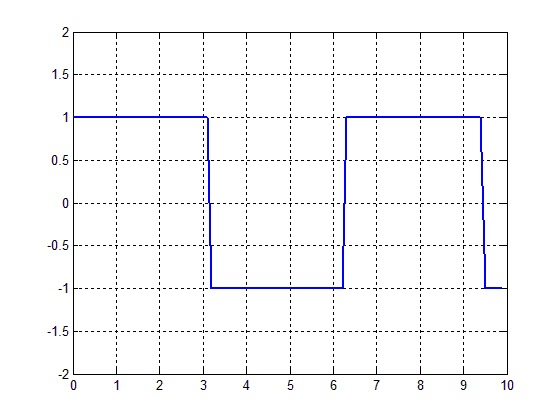
\includegraphics[width=6.5cm]{5_3} 
    \caption{Полигармонический сигнал}\label{fig.l5_3}}
  \hfil\hfil 
  \begin{minipage}[b]{0.49\textwidth}
	\centering
	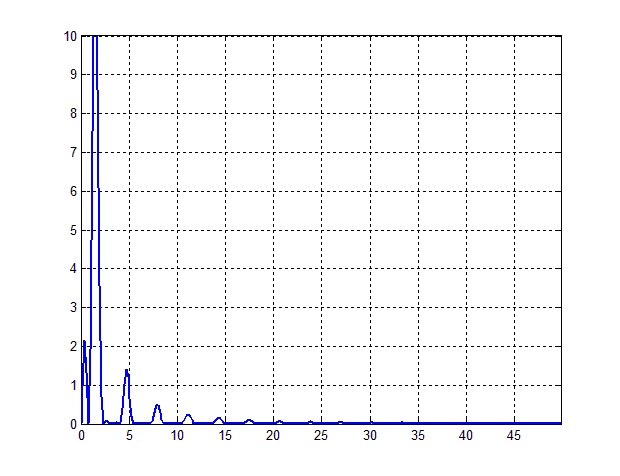
\includegraphics[width=6.5cm]{5_4}
	\caption{Спектр полигармонического сигнала}\label{fig.l5_4} 
  \end{minipage}
\end{figure}

\begin{figure}[h]\centering
  \parbox[b]{0.49\textwidth}{\centering
    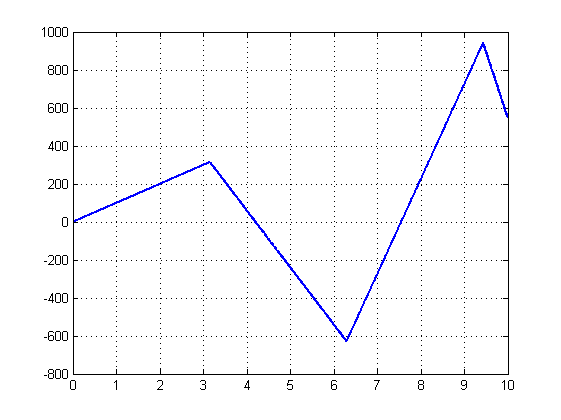
\includegraphics[width=6.5cm]{5_5} 
    \caption{Полигармонический сигнал}\label{fig.l5_5}}
  \hfil\hfil 
  \begin{minipage}[b]{0.49\textwidth}
	\centering
	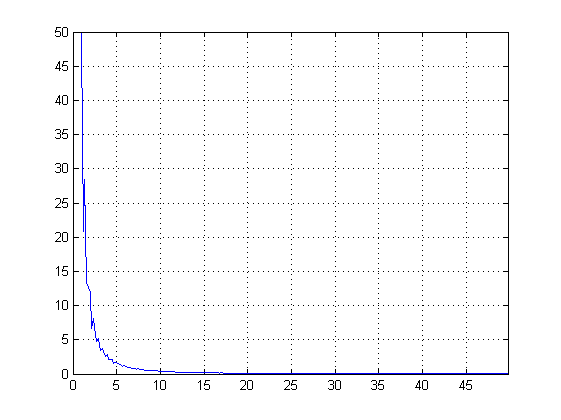
\includegraphics[width=6.5cm]{5_6}
	\caption{Спектр полигармонического сигнала}\label{fig.l5_6} 
  \end{minipage}
\end{figure}

\FloatBarrier

В ходе моделирования сигналов в Simulink были собраны следующие схемы и получены соответствующие графики:


\begin{itemize}
\item Полигармонический сигнал (Рис. 11 - 13)
\begin{figure}[h]
\centering
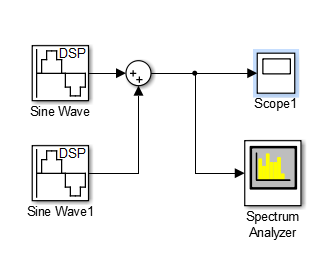
\includegraphics[width=10cm]{1_simulink} 
\caption{Полигармонический сигнал (Simulink)} 
\label{fig.l5_1s} 
\end{figure}
\begin{figure}[h]
\centering
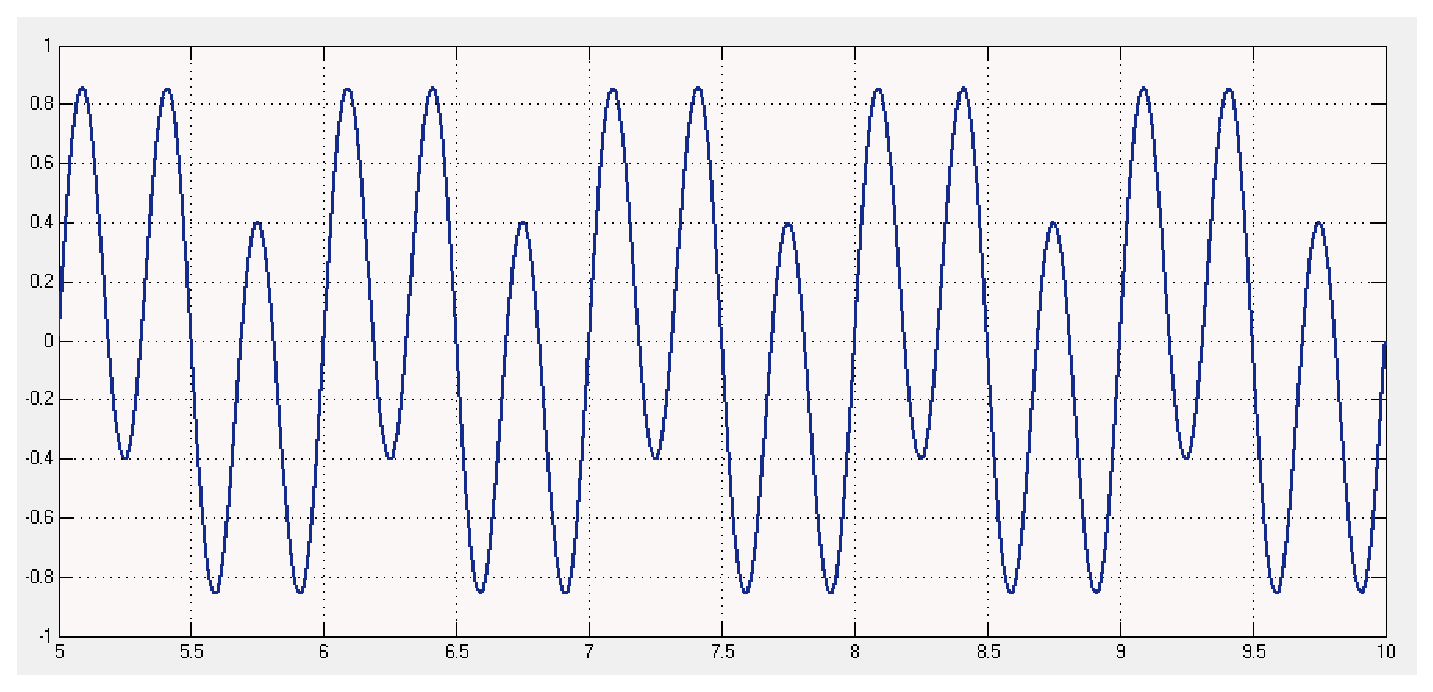
\includegraphics[width=10cm]{lab5_1_simulink} 
\caption{Полигармонический сигнал} 
\label{fig.l5_2s1} 
\end{figure}
\begin{figure}[h]
\centering
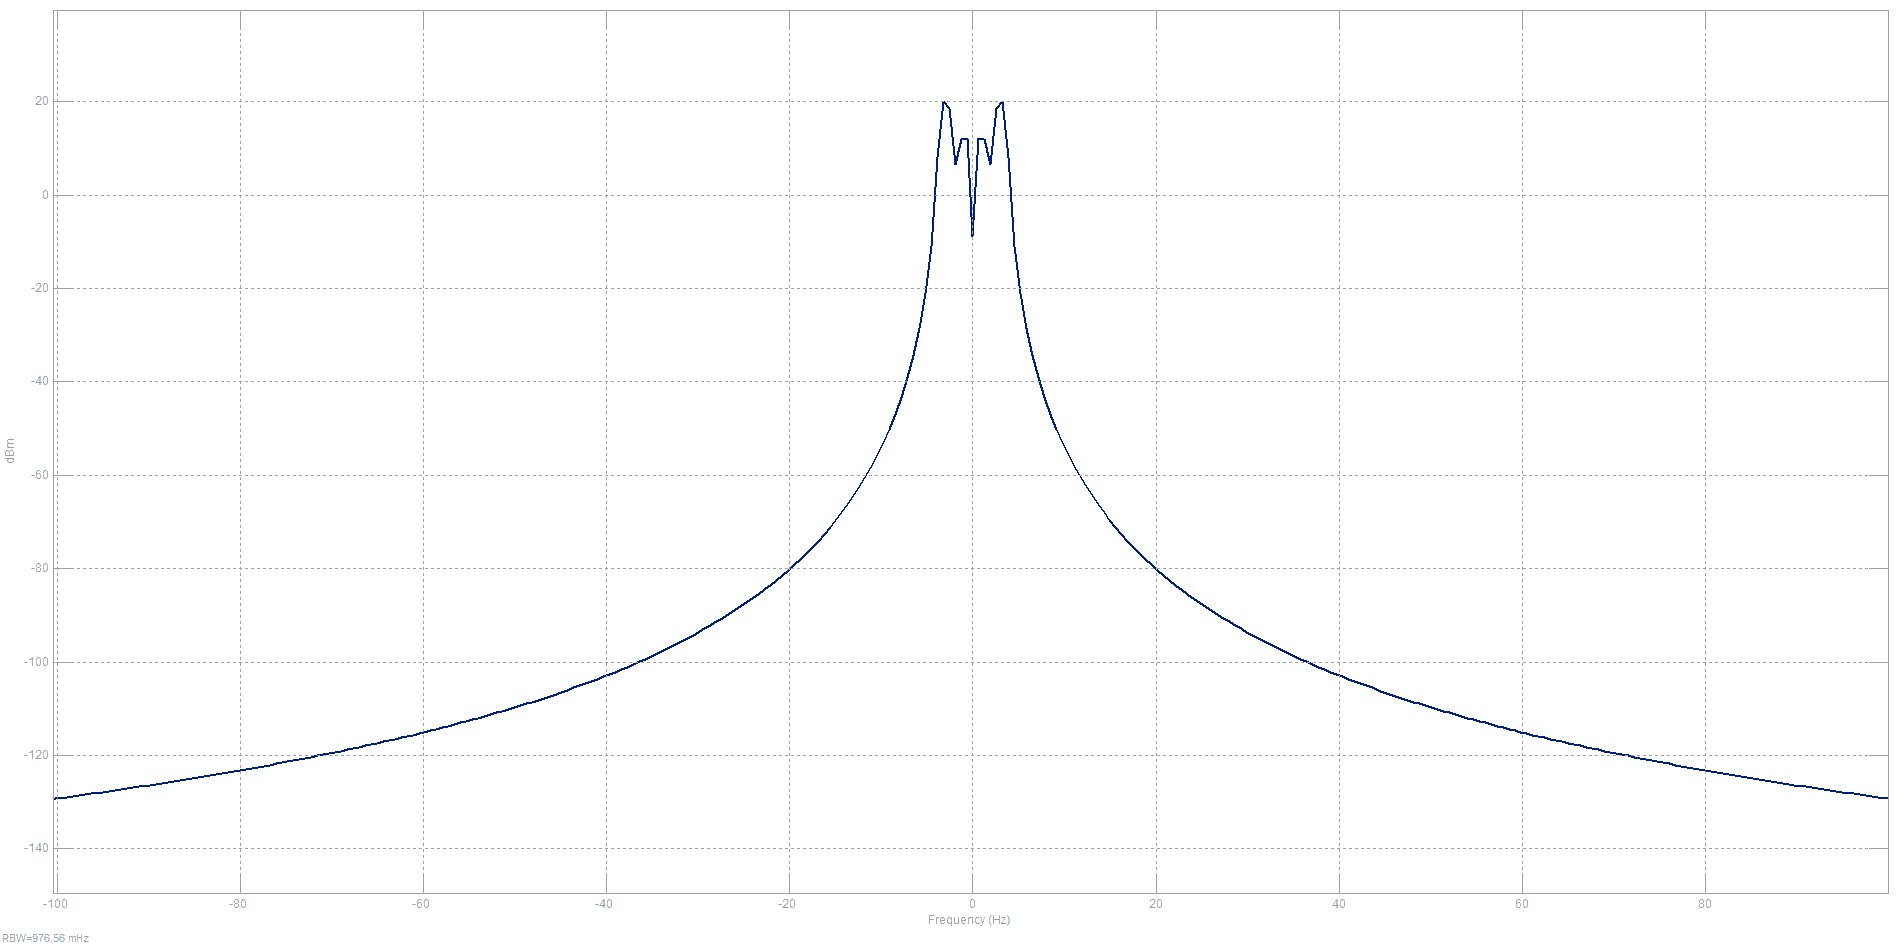
\includegraphics[width=10cm]{lab5_2_simulink}
\caption{Спектр полигармонического сигнала} 
\label{fig.l5_3s} 
\end{figure}

\item Прямоугольный импульсный сигнал (Рис. 14 - 16)
\begin{figure}[h]
\centering
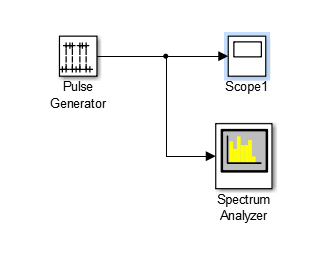
\includegraphics[width=10cm]{3_simulink} 
\caption{Прямоугольный импульсный сигнал (Simulink)} 
\label{fig.l5_4s} 
\end{figure}
\begin{figure}[h]
\centering
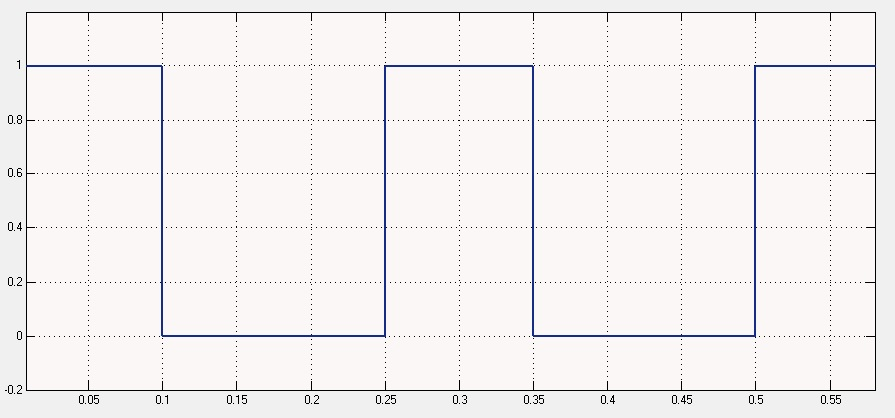
\includegraphics[width=10cm]{lab5_3_simulink} 
\caption{Прямоугольный импульсный сигнал} 
\label{fig.l5_5s} 
\end{figure}
\begin{figure}[h]
\centering
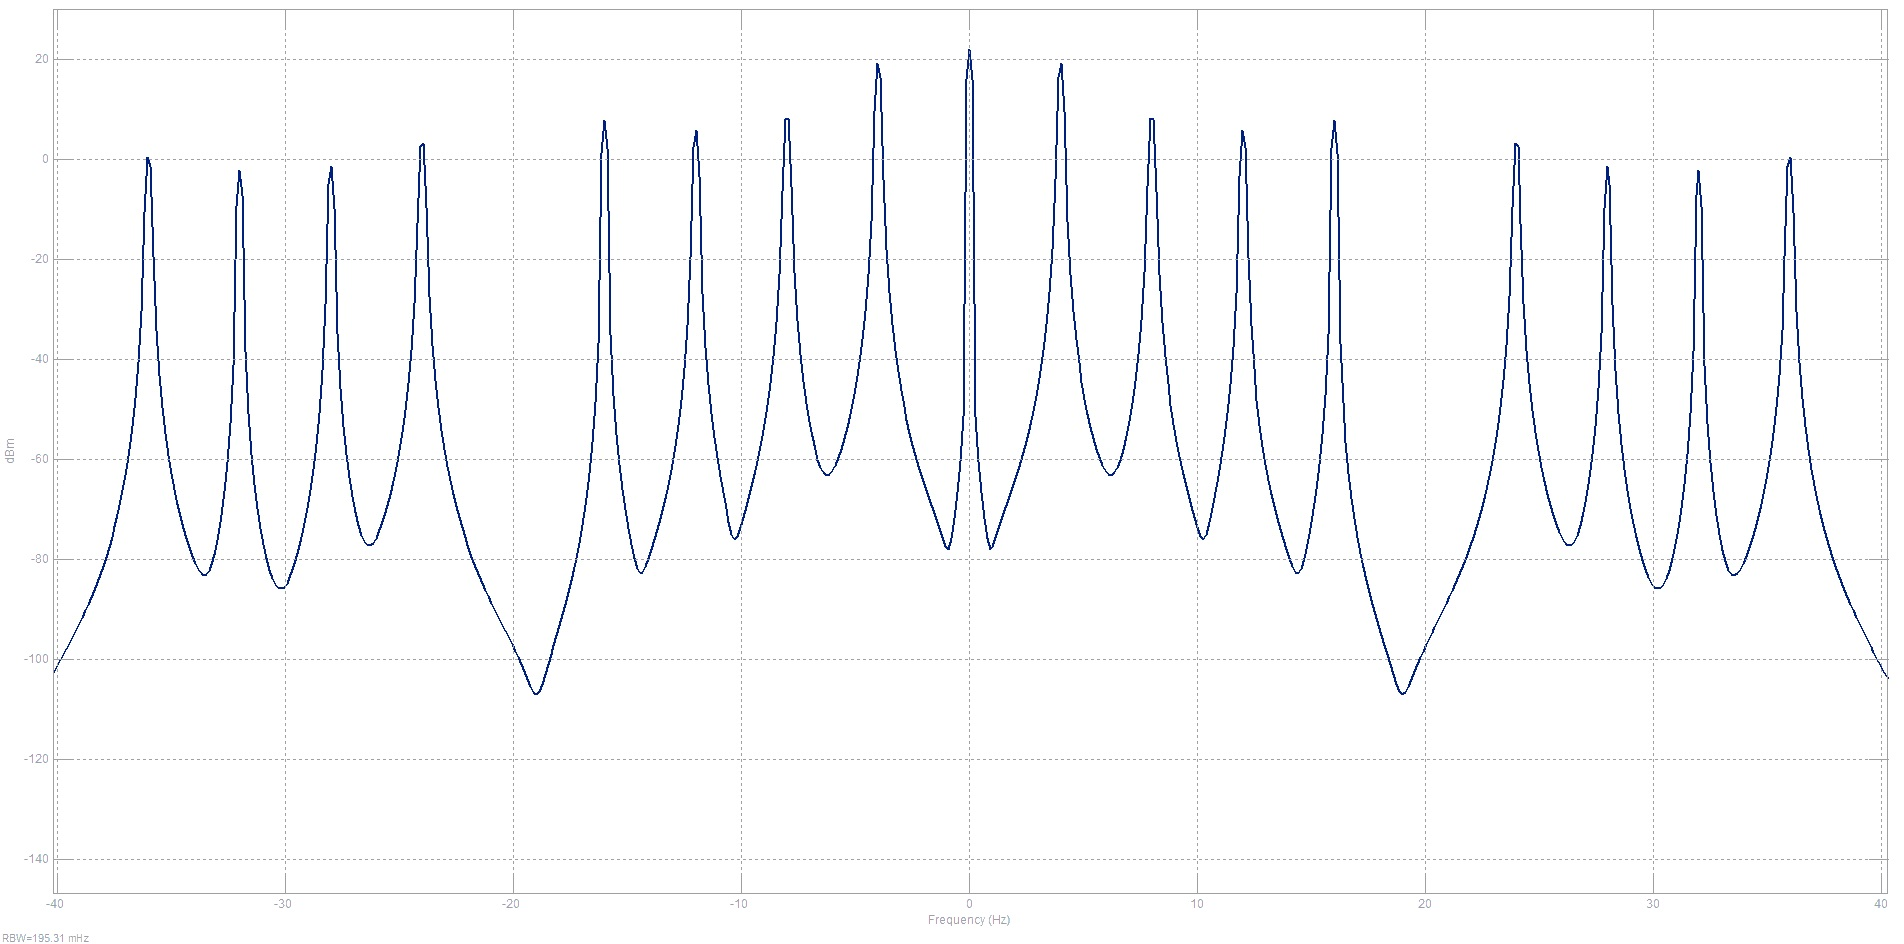
\includegraphics[width=10cm]{lab5_4_simulink}
\caption{Спектр прямоугольного сигнала} 
\label{fig.l5_6s} 
\end{figure}

\item Треугольный импульсный сигнал (Рис. 17 - 19)
\begin{figure}[h]
\centering
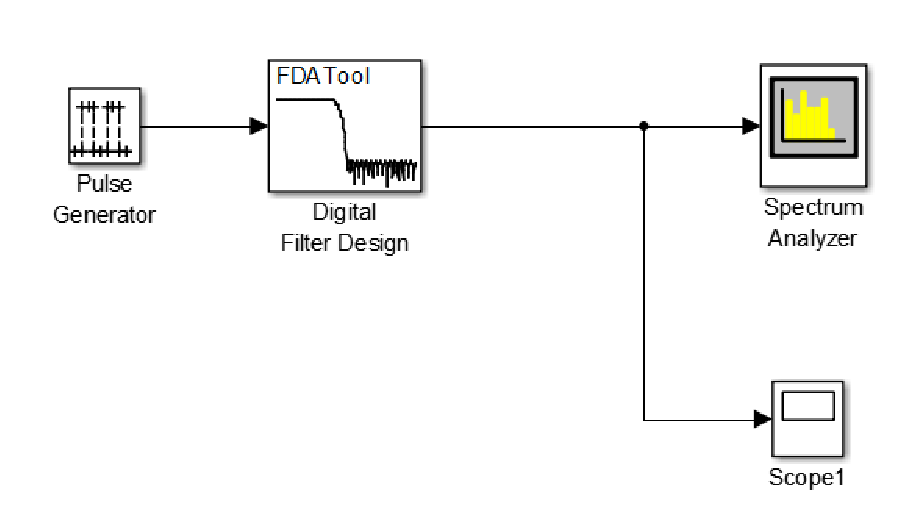
\includegraphics[width=10cm]{4_simulink} 
\caption{Треугольный импульсный сигнал (Simulink)} 
\label{fig.l5_7s} 
\end{figure}
\begin{figure}[h]
\centering
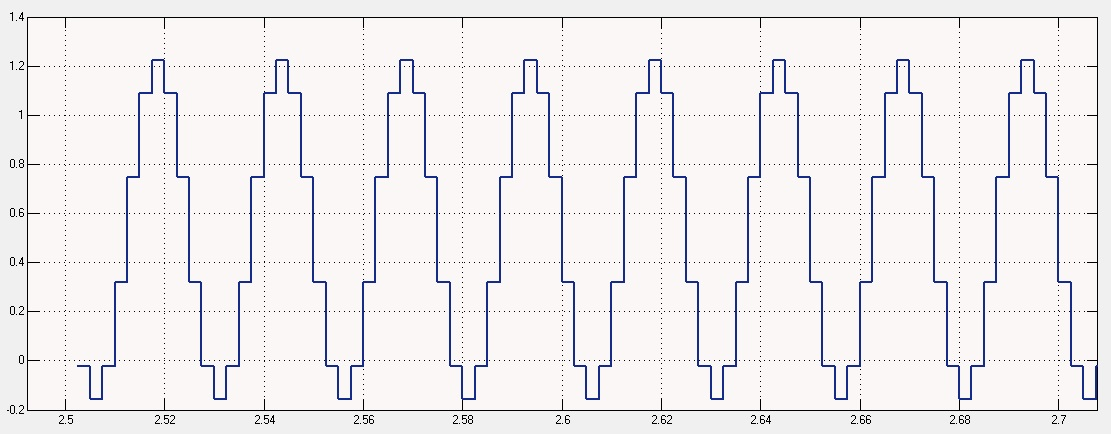
\includegraphics[width=10cm]{lab5_5_simulink} 
\caption{Треугольный импульсный сигнал} 
\label{fig.l5_8s} 
\end{figure}
\begin{figure}[h]
\centering
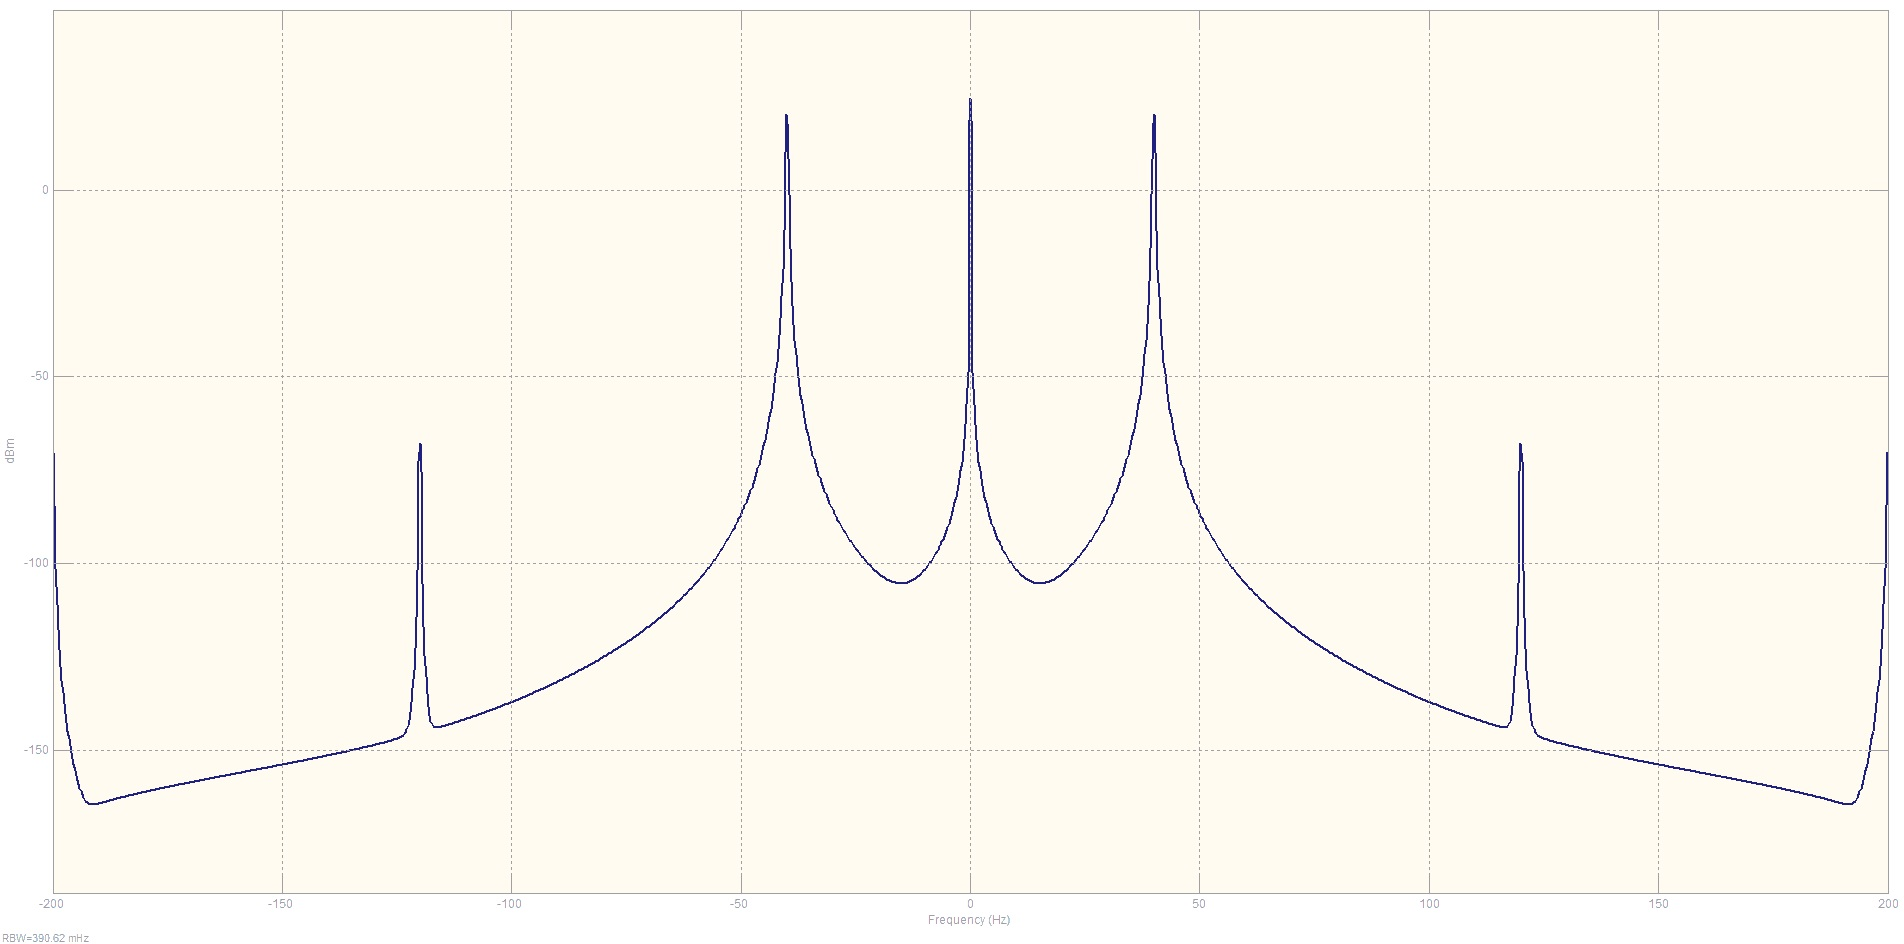
\includegraphics[width=10cm]{lab5_6_simulink}
\caption{Спектр треугольного сигнала} 
\label{fig.l5_9s} 
\end{figure}
\end{itemize}
\FloatBarrier
\subsection{Выводы}
В результате проделанной работы было проведено моделирование в среде MatLAB и Simulink полигармонического, прямоугольного и треугольного импульсных сигналаов, а также получены их спектры. В Simulink для получения генератора треугольного сигнала используется генератор прямоугольных импульсов каскадно с фильтром с прямоугольным окном. Это обоснуется тем, что свертка двух прямоугольных импульсов в результате дает треугольный.

\newpage
\section{Линейная фильтрация}

\subsection{Цель работы}
Изучить воздействие ФНЧ на тестовый сигнал с шумом.

\subsection{Постановка задачи}
Сгенерировать гармонический сигнал с шумом и синтезировать ФНЧ. Получить сигнал во временной и частотной областях до и после фильтрации. Сделать выводы о воздействии ФНЧ на спектр сигнала.

\subsection{Справочные материалы}
В.С. Гутников. Фильтрация измерительных сигналов пп. 17-19

\subsection{Ход работы}
Фильтрация сигнала - изменение его спектра, которое обычно применяется с целью увеличить отношение полезного сигнала к шумам и помехам или усилить какие-нибудь полезные качества сигнала.
В данной работе рассматривается фильтр нижних частот (ФНЧ), пропускающий низкочастотные составляющие спектра и задерживают высокочастотные, а именно фильтр Баттерворта с максимально гладкой АЧХ.  
Для моделирования заданных сигналов использовался приведенный ниже код MATLAB:
\begin{flushleft}

x = 0:0.01:4*pi;\\
f = 100*(0:255)/512;\\

noise = rand(size(x));\\
y = sin(2*pi*x);            \% Сигнал без шума\\
y\_noisy = y+0.3*noise;      \% Сигнал с шумом\\

figure\\
plot(x(1:200),y(1:200))\\
grid\\

figure\\
plot(x(1:200),y\_noisy(1:200))\\
grid\\

[B,A] = butter(16,0.98);    \% Синтез ФНЧ Баттерворта\\
B = B./sum(B);\\
A = A./sum(A);\\
                      
y\_filtered = conv(y\_noisy, [B, A]); \% Обработка сигнала ФНЧ\\

figure\\
plot(x(1:200),y\_filtered(1:200))\\
grid\\

noisy\_spectrum = fft(y\_noisy, 512); \% Спектр сигнала с шумом\\
norm\_noisy\_spectrum = noisy\_spectrum.*conj(noisy\_spectrum)/512;\\

figure\\
plot(f, norm\_noisy\_spectrum(1:256))\\
axis([0 max(f) 0 2])\\
grid \\

filtered\_spectrum = fft(y\_filtered, 512);   \% Спектр фильтрованного сигнала\\
norm\_filtered\_spectrum = filtered\_spectrum.*conj(filtered\_spectrum)/512;\\

figure\\
plot(f, norm\_filtered\_spectrum(1:256))\\
axis([0 max(f) 0 2])\\
grid\\


\end{flushleft}
\subsection{Результаты работы}
В результате работы представленного кода были получены следующие данные:

\begin{itemize}
\item Исходный гармонический сигнал (Рис. 20); 
\item Сигнал с шумом и его спектр (Рис. 21 - 22);
\item Отфильтрованный сигнал и его спектр (Рис. 23 - 24).
\end{itemize}

\begin{figure}[h]
\centering
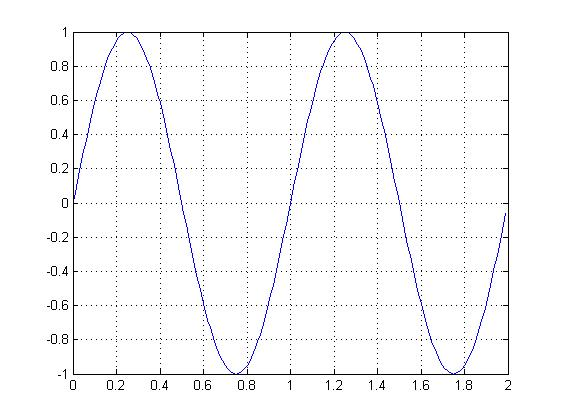
\includegraphics[width=6.5cm]{lab6_0} 
\caption{Исходный гармонический сигнал} 
\label{fig.l6_0} 
\end{figure}

\begin{figure}[h]\centering
  \parbox[b]{0.49\textwidth}{\centering
    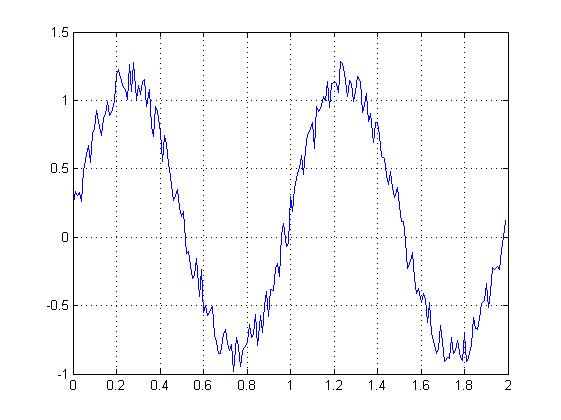
\includegraphics[width=6.5cm]{lab6_1} 
    \caption{Зашумленный гармонический сигнал}\label{fig.l6_1}}
  \hfil\hfil 
  \begin{minipage}[b]{0.49\textwidth}
	\centering
	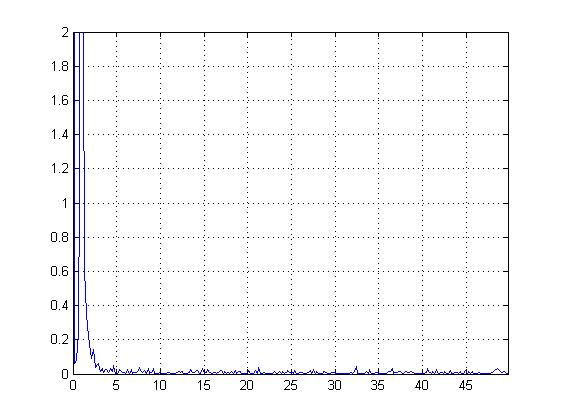
\includegraphics[width=6.5cm]{lab6_2}
	\caption{Спектр зашумленного сигнала}\label{fig.l6_2} 
  \end{minipage}
\end{figure}

\begin{figure}[h]\centering
  \parbox[b]{0.49\textwidth}{\centering
    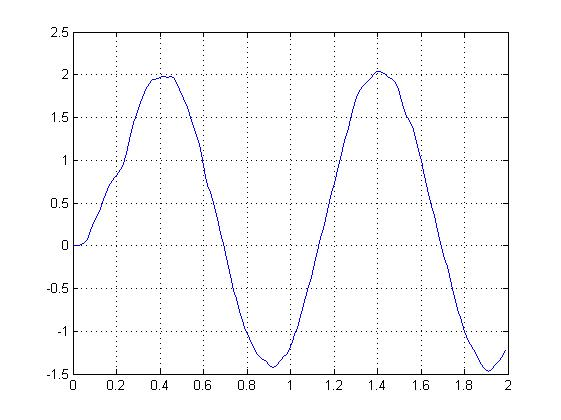
\includegraphics[width=6.5cm]{lab6_3} 
    \caption{Отфильтрованный сигнал}\label{fig.l6_3}}
  \hfil\hfil 
  \begin{minipage}[b]{0.49\textwidth}
	\centering
	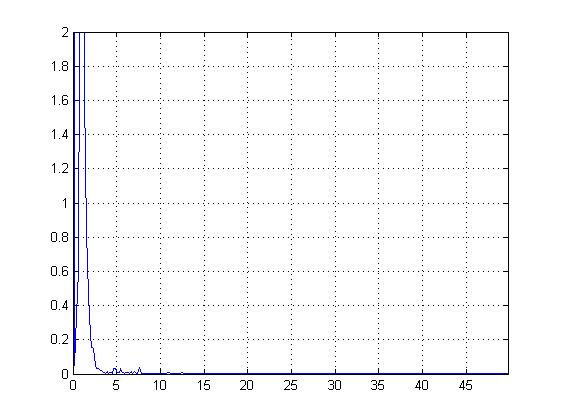
\includegraphics[width=6.5cm]{lab6_4}
	\caption{Спектр отфильтрованного сигнала}\label{fig.l6_4} 
  \end{minipage}
\end{figure}

\FloatBarrier
                                                                                                                                                                                                                                                                                                                                                                                                                                                                                                                                                                                                                                                                                                                                                                                                                                                                                                                                                                                                                                                                                                                                                                                                                                                                                                                                                                                                                                                                                                                                                                                                                                                                                                                                                                                                                                                                                                                                                                                                                                                                                                                                                                                                                                                                                                                                                                                                                                                                                                                                                                                                                                                                                                                                                                                                                                                                                                                                                                                                                                                                                                                                                                                                                                                                                                                                                                                                                                                                                                                                                                                                                                                                                                                                                                                                                                                                                                                                                                                                                                                                                                                                                                                                                                                              Аналогичное моделирование было проведено в среде Simulink (построенный блок отображен на Рис. 25). В результате были получены характеристики, представленные на Рис. 26 - 27.
                                                                                                                                                                                                                                                                                                                                                                                                                                                                                                                                                                                                                                                                                                                                                                                                                                                                                                                                                                                                                                                                                                                                                                                                                                                                                                                                                                                                                                                                                                                                                                                                                                                                                                                                                                                                                                                                                                                                                                                                                                                                                                                                                                                                                                                                                                                                                                                                                                                                                                                                                                                                                                                                                                                                                                                                                                                                                                                                                                                                                                                                                                                                                                                                                                                                                                                                                                                                                                                                                                                                                                                                                                                                                                                                                                                                                                                                                                                                                                                                                                                                                                                                                                                                                                                               \begin{figure}[h]\centering
	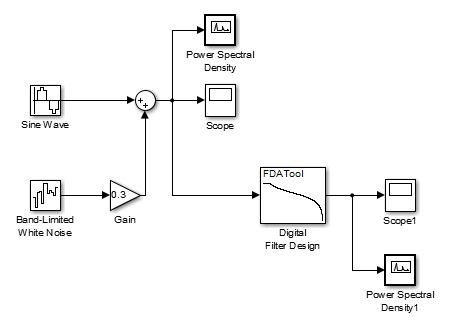
\includegraphics[width=10cm]{Sim_0} 
	\caption{Исходный гармонический сигнал}\label{fig.l6_Sim0} 
\end{figure}
                                                                                                                                                                                                                                                                                                                                                                                                                                                                                                                                                                                                                                                                                                                                                                                                                                                                                                                                                                                                                                                                                                                                                                                                                                                                                                                                                                                                                                                                                                                                                                                                                                                                                                                                                                                                                                                                                                                                                                                                                                                                                                                                                                                                                                                                                                                                                                                                                                                                                                                                                                                                                                                                                                                                                                                                                                                                                                                                                                                                                                                                                                                                                                                                                                                                                                                                                                                                                                                                                                                                                                                                                                                                                                                                                                                                                                                                                                                                                                                                                                                                                                                                                                                                                                                               \begin{figure}[h]\centering
    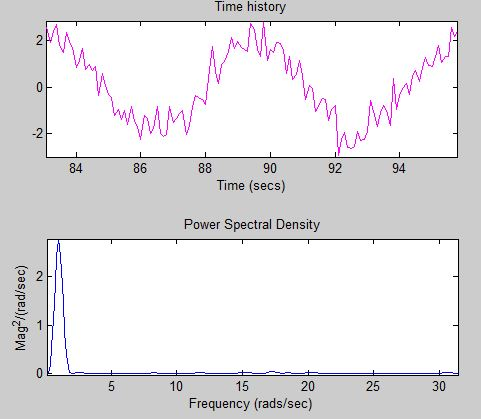
\includegraphics[width=10cm]{Sim_1} 
    \caption{Отфильтрованный сигнал}\label{fig.l6_Sim1}
\end{figure}

\begin{figure}\centering
	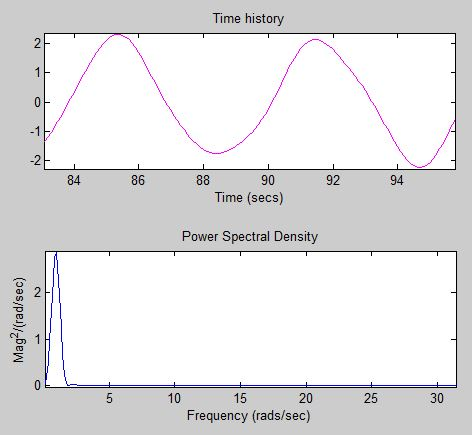
\includegraphics[width=10cm]{Sim_2}
	\caption{Спектр отфильтрованного сигнала}\label{fig.l6_Sim2}
\end{figure}                                                                                                                                                                                                                                                                                                                                                                                                                                                                                                                                                                                                                                                                                                                                                                                                                                                                                                                                                                                                                                                                                                                                                                                                                                                                                                                                                                                                                                                                        

\FloatBarrier

\subsection{Выводы}
В данной работе было изучено воздействие ФНЧ на тестовый сигнал с шумом, а именно произведено зашумление и удаление шума линейым фильтром Баттерворта. Однако фильтрация оказалась неполной. Это связано с тем, что использованный линейный фильтр не способен разделить шум и полезный сигнал в одной частотной области. Для полной фильтрации необходимо использовать идеальный фильтр с прямоугольным окном.

\newpage
\section{Аналоговая модуляция}

\subsection{Цель работы}
Изучение аналоговой модуляции/демодуляции сигнала.

\subsection{Постановка задачи}
	\begin{enumerate}
		\item Сгенерировать однотоальный сигнал низкой частоты.
		\item Выполнить амплитудную модуляцию сигнала по закону
				\begin{equation}
					u(t) = (1+MU_m cos(\Omega t))cos(\omega_0 t+\phi_0).
				\end{equation}
		\item Получить спектр модулированного сигнала.
		\item Выполнить модуляцию с подавлением несущей 
				\begin{equation}
					u(t) = MU_m cos(\omega t)cos(\omega_0 t+\phi_0).
				\end{equation}
		      Получить спектр. 
		\item Выполнить однополосную модуляцию:
				\begin{equation}
					u(t) = U_m cos(\omega t)cos(\omega_0 t+\phi_0)+\frac{U_m}{2}\sum_{n=1}^N M_n (cos(\omega_0 + \Omega_n )t + \phi_0 + \Phi_n ),
				\end{equation}
				положив n = 1.
		\item Выполить синхронное детектирование и получить исходный однополосный сигнал.
		\item Рассчитать КПД модуляции
				\begin{equation}
					\eta_A M = \frac{U_m ^2 M^2 /4}{P_U} = \frac{M^2}{M^2 + 2}.
				\end{equation}
	\end{enumerate}

\subsection{Справочные материалы}
Н.В. Богач и др. Обработка сигналов в информационных системах, с. 110-118, 125-127.

\subsection{Ход работы}
АМ - сигнал представляет собой произведение информационной огибающей u(t) и гармонического колебания ее заполнения с более высокими частотами. Простейшая форма модулированного сигнала создается при \textit{однотональной} АМ - модуляции несущего сигнала гармоническим колебанием с одной частотой $\Omega$:
	\begin{equation}
		u(t) = (1+MU_m cos(\Omega t))cos(\omega_0 t+\phi_0).
	\end{equation}

Реализация аналоговой модуляции с помощью MATLAB:
\begin{flushleft}
x = 0:0.01:4*pi;\\
f0 = 0.2;\\

\% Исходный сигнал\\
y = sin(2*pi*f0*x);\\
figure\\
plot(x(1:500),y(1:500), 'LineWidth', 2)\\
grid\\

\% Спектр исходного сигнала\\
spectrum = fft(y, 512);\\
norm\_spectrum = spectrum.*conj(spectrum)/512;\\
f = 100*(0:255)/512;\\
figure\\
plot(f, norm\_spectrum(1:256), 'LineWidth', 2)\\
axis([0 max(f) 0 40])\\
grid\\

\% Амплитудная модуляция\\
Fc = 5*f0;\\
Fs = 50*f0;\\
U = ammod(y, Fc, Fs, 0, 1);\\
figure \\
plot(x(1:500), U(1:500))\\
grid\\

\% Спектр модурированного сигнала\\
u\_spectrum = fft(U, 512);\\
norm\_u\_spectrum = u\_spectrum.*conj(u\_spectrum)/512;\\
figure\\
plot(f, norm\_u\_spectrum(1:256))\\
axis([0 max(f) 0 30])\\
grid\\
\end{flushleft}

В результате выполнения приведенного кода были получены следующие характеристики:

\begin{figure}[h]\centering
  \parbox[b]{0.49\textwidth}{\centering
    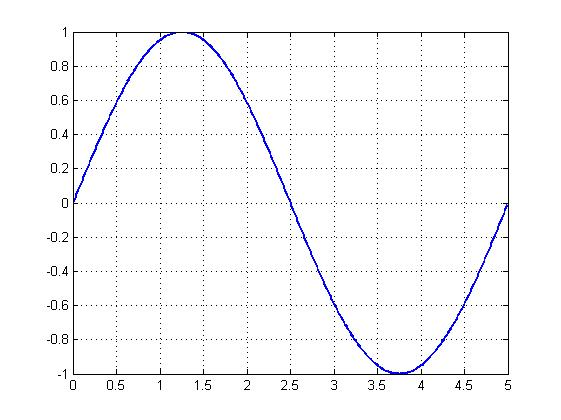
\includegraphics[width=6.5cm]{lab7_0} 
    \caption{Исходный гармонический сигнал}\label{fig.l7_0}}
  \hfil\hfil 
  \begin{minipage}[b]{0.49\textwidth}
	\centering
	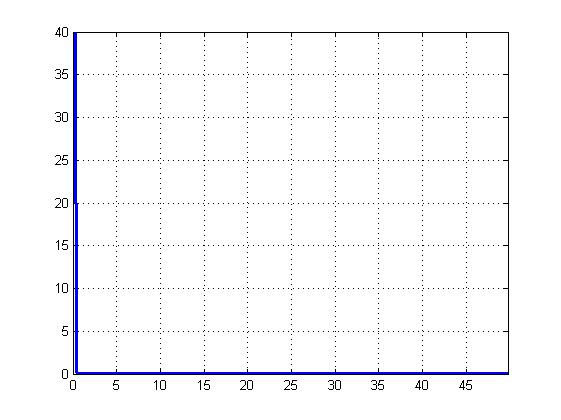
\includegraphics[width=6.5cm]{lab7_1}
	\caption{Спектр исходного сигнала}\label{fig.l7_1} 
  \end{minipage}
\end{figure}

\begin{figure}[h]\centering
  \parbox[b]{0.49\textwidth}{\centering
    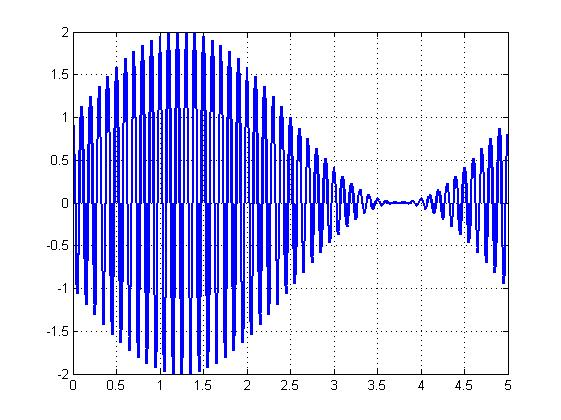
\includegraphics[width=6.5cm]{lab7_2} 
    \caption{Модуляция с М = 1}\label{fig.l7_2}}
  \hfil\hfil 
  \begin{minipage}[b]{0.49\textwidth}
	\centering
	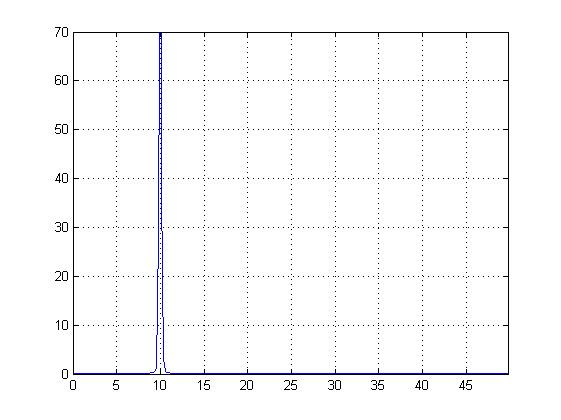
\includegraphics[width=6.5cm]{lab7_3}
	\caption{Спектр АМ-сигнала (М = 1)}\label{fig.l7_3} 
  \end{minipage}
\end{figure}

\begin{figure}[h]\centering
  \parbox[b]{0.49\textwidth}{\centering
    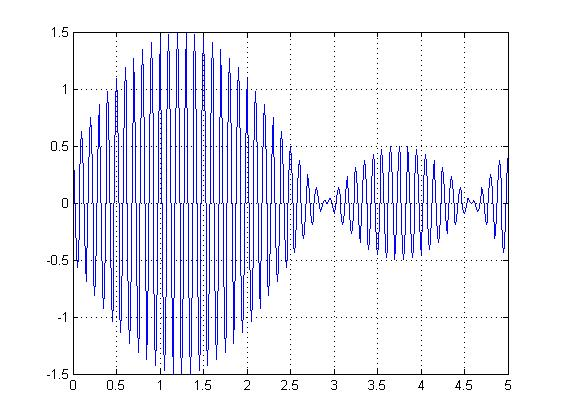
\includegraphics[width=6.5cm]{lab7_4} 
    \caption{Модуляция с М = 2}\label{fig.l7_4}}
  \hfil\hfil 
  \begin{minipage}[b]{0.49\textwidth}
	\centering
	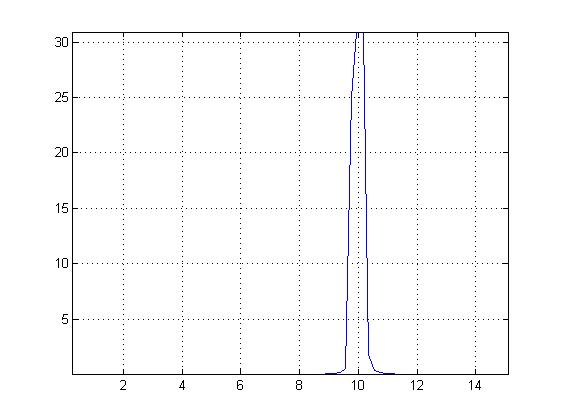
\includegraphics[width=6.5cm]{lab7_5}
	\caption{Спектр АМ-сигнала (М = 2)}\label{fig.l7_5} 
  \end{minipage}
\end{figure}

\begin{figure}[h]\centering
  \parbox[b]{0.49\textwidth}{\centering
    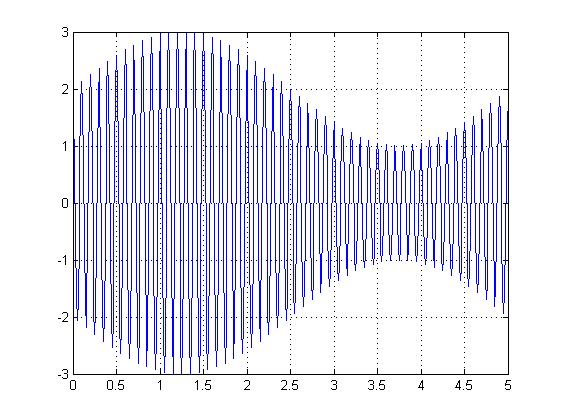
\includegraphics[width=6.5cm]{lab7_6} 
    \caption{Модуляция с М = 0.5}\label{fig.l7_6}}
  \hfil\hfil 
  \begin{minipage}[b]{0.49\textwidth}
	\centering
	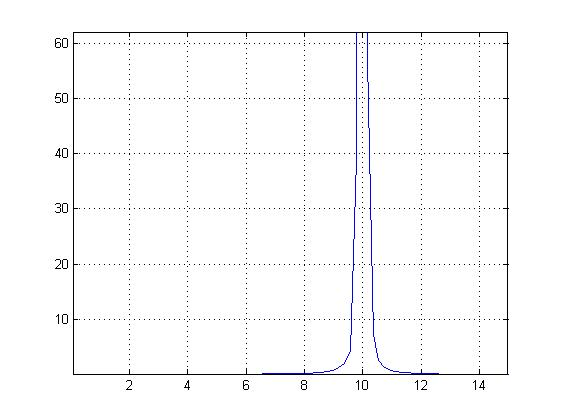
\includegraphics[width=6.5cm]{lab7_7}
	\caption{Спектр АМ-сигнала (М = 0.5)}\label{fig.l7_7} 
  \end{minipage}
\end{figure}

\FloatBarrier

При балансной модуляции (АМ с подавлением несущей) производится перемножение двух сигналов - модулирующего и несущего, при котором проиходит подавление неcущего колебания, соответственно, КПД модуляции становится равным 100\%. 
Физическая сущность подавления несущей заключается в том, что при переходе огибающей биений U(t) через 0 фаза несущей частоты высокочастотного заполнения изменяется на $180^0$.

Реализация аналоговой модуляции c подавлением несущей с помощью MATLAB:
\begin{flushleft}

\% Амплитудная модуляция с подавлением несущей\\
Fc = 10*f0;\\
Fs = 100*f0;\\
U = ammod(y, Fc, Fs);\\
figure \\
plot(x(1:500), U(1:500), 'LineWidth', 2)\\
grid\\

\% Спектр модурированного сигнала\\
u\_spectrum = fft(U, 512);
norm\_u\_spectrum = u\_spectrum.*conj(u\_spectrum)/512;\\
figure\\
plot(f, norm\_u\_spectrum(1:256))\\
axis([0 max(f) 0 30])\\
grid\\
\end{flushleft}

В результате выполнения приведенного кода были получены следующие характеристики:

\begin{figure}[h]\centering
  \parbox[b]{0.49\textwidth}{\centering
    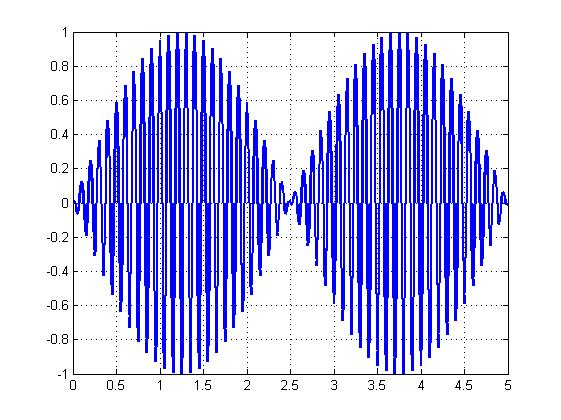
\includegraphics[width=6.5cm]{lab7_8} 
    \caption{АМ-сигнал с подавлением несущей}\label{fig.l7_8}}
  \hfil\hfil 
  \begin{minipage}[b]{0.49\textwidth}
	\centering
	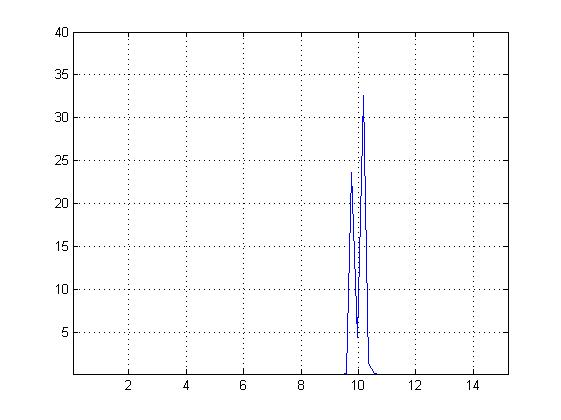
\includegraphics[width=6.5cm]{lab7_9}
	\caption{Спектр АМ-сигнала с подавлением}\label{fig.l7_9} 
  \end{minipage}
\end{figure}

\FloatBarrier

Спектры двух боковых полос АМ-сигнала являются зеркальным отражением друг друга, т.е. они несут одну и ту же информацию. Поэтому одну из боковых полос можно удалить.

Для этого был использван следующий код MATLAB:
\begin{flushleft}
\% Однополосная амплитудная модуляция\\
Fc = 10*f0;\\
Fs = 100*f0;\\
U = ssbmod(y, Fc, Fs, [], 'upper');\\
figure \\
plot(x(1:500), U(1:500), 'LineWidth', 2)\\
grid\\

\% Спектр модурированного сигнала\\
u\_spectrum = fft(U, 512);
norm\_u\_spectrum = u\_spectrum.*conj(u\_spectrum)/512;\\
figure\\
plot(f, norm\_u\_spectrum(1:256))\\
axis([0 max(f) 0 30])\\
grid\\
\end{flushleft}

В результате выполнения приведенного кода были получены следующие графики:

\begin{figure}[h]\centering
  \parbox[b]{0.49\textwidth}{\centering
    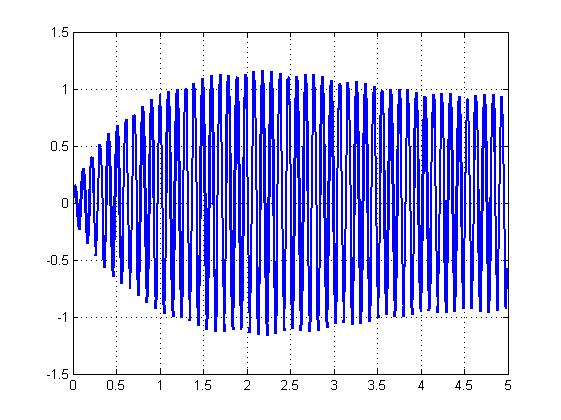
\includegraphics[width=6.5cm]{lab7_10} 
    \caption{Однополосный АМ-сигнал}\label{fig.l7_10}}
  \hfil\hfil 
  \begin{minipage}[b]{0.49\textwidth}
	\centering
	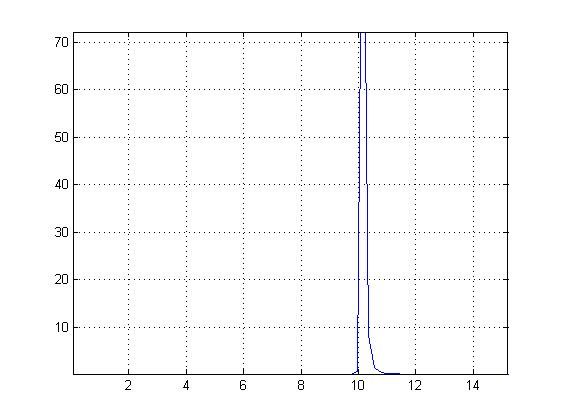
\includegraphics[width=6.5cm]{lab7_11}
	\caption{Спектр однополосного АМ-сигнала}\label{fig.l7_11} 
  \end{minipage}
\end{figure}

\FloatBarrier

Синхронное детектирование является одним из способов демодуляции АМ-сигнала. Его суть состоит в умножении частоты сигнала на опорное колебание с несущей частотой. Результат умножения содержит два слагаемых: искомая амплитуда и АМ-сигнал с несущей частотой $2\omega_0$, который легко удаляется путем пропускания сигнала через ФНЧ.

Ниже приведен реализующий синхронное детектирование код MATLAB:

\begin{flushleft}
\% Синхронное детектирование\\
%[b,a] = butter(10, Fc*2/Fs);\\
z = ssbdemod(U, Fc, Fs, 0, b, a);\\
figure\\
plot(x(1:1000), z(1:1000))\\
grid\\

\% Спектр демодулированного сигнала\\
du\_spectrum = fft(U, 512);\\
norm\_du\_spectrum = du\_spectrum.*conj(du\_spectrum)/512;\\
figure\\
plot(f, norm\_du\_spectrum(1:256))\\
axis([0 max(f) 0 70])\\
grid\\
\end{flushleft}

В результате синхронного дететирования демодулированный сигнал полностью совпал с исходным сигналом:

\begin{figure}[h]\centering
  \parbox[b]{0.49\textwidth}{\centering
    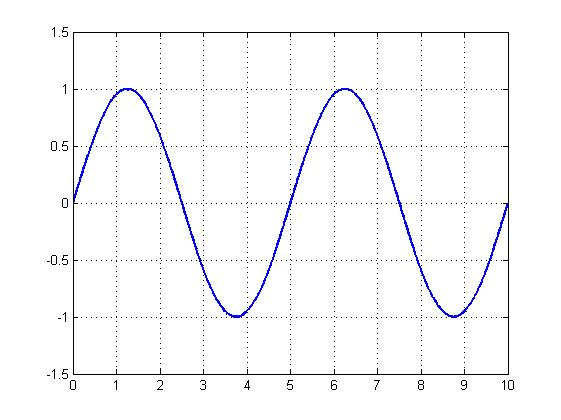
\includegraphics[width=6.5cm]{lab7_12} 
    \caption{Демодулированный АМ-сигнал}\label{fig.l7_12}}
  \hfil\hfil 
  \begin{minipage}[b]{0.49\textwidth}
	\centering
	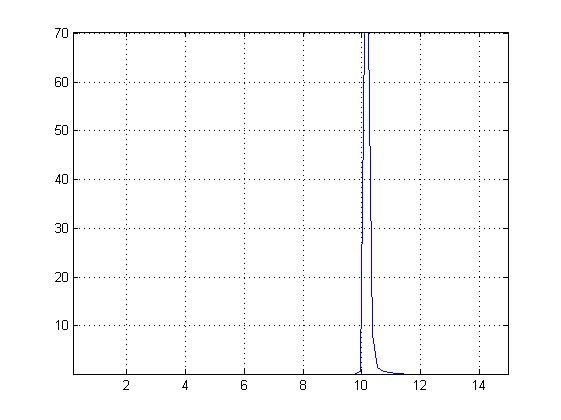
\includegraphics[width=6.5cm]{lab7_13}
	\caption{Спектр демодулированного сигнала}\label{fig.l7_13} 
  \end{minipage}
\end{figure}

\FloatBarrier

В ходе работы был рассчитан КПД модуляции при различных значениях глубины М:

\begin{itemize}
	\item M = 1:		0.33;
	\item M = 2:		0.67;
	\item M = 0.5:		0.11.
\end{itemize}

\textbf{Однополосная модуляция/демодуляция в среде Simulink}

Для моделирования амплитудной однополосной модуляции и демодуляции использовались блоки SSB AM Modulator/Demodulaor Passband. Результаты моделирования приведены на Рис. 42-45:

\begin{figure}[h]\centering
	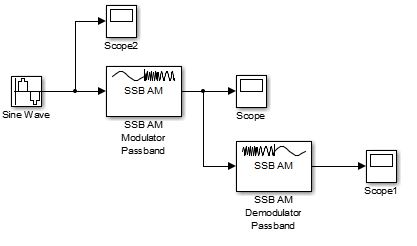
\includegraphics[width=6cm]{Sim_ssb0}
	\caption{Схема однополосной модуляции/демодуляции}\label{fig.Sim_ssb0}
\end{figure}                                                                                                                                                                                                                                                                                                                                                                                                                                                                                                                                                                                                                                                                                                                                                                                                                                                                                                                                                                                                                                                                                                                                                                                                                                                                                                                                                                                                                                                                        

\begin{figure}[h]\centering
	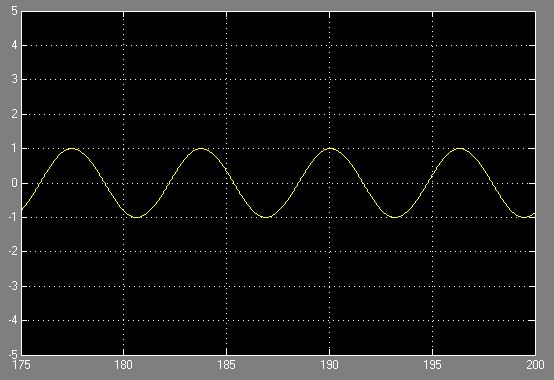
\includegraphics[width=8cm]{Sim_ssb1}
	\caption{Исходный сигнал}\label{fig.Sim_ssb1}
\end{figure}                                                                                                                                                                                                                                                                                                                                                                                                                                                                                                                                                                                                                                                                                                                                                                                                                                                                                                                                                                                                                                                                                                                                                                                                                                                                                                                                                                                                                                                                        

\begin{figure}[h]\centering
	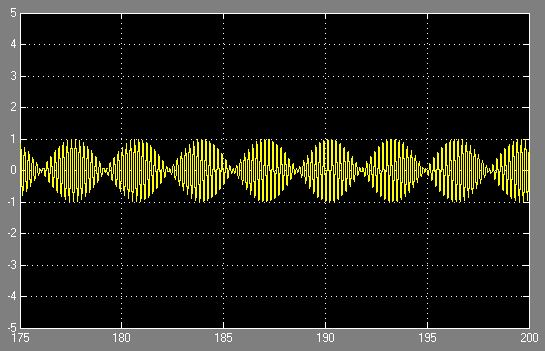
\includegraphics[width=8cm]{Sim_ssb2}
	\caption{АМ-сигнал}\label{fig.Sim_ssb2}
\end{figure}                                                                                                                                                                                                                                                                                                                                                                                                                                                                                                                                                                                                                                                                                                                                                                                                                                                                                                                                                                                                                                                                                                                                                                                                                                                                                                                                                                                                                                                                        

\begin{figure}[h]\centering
	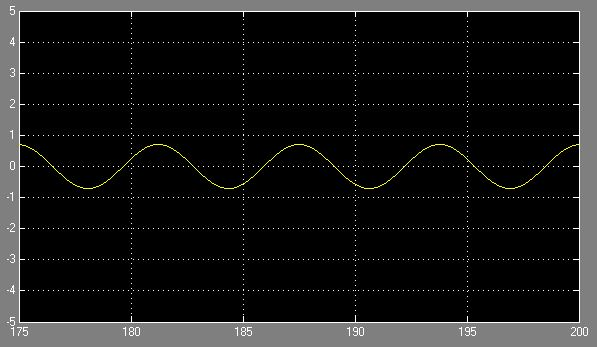
\includegraphics[width=8cm]{Sim_ssb3}
	\caption{Демодулированный АМ-сигнал}\label{fig.Sim_ssb3}
\end{figure}                                                                                                                                                                                                                                                                                                                                                                                                                                                                                                                                                                                                                                                                                                                                                                                                                                                                                                                                                                                                                                                                                                                                                                                                                                                                                                                                                                                                                                                                        

\FloatBarrier

Для моделирования балансной однополосной модуляции и демодуляции использовались блоки DSBSC AM Modulator/Demodulaor Passband. Исходный сигнал тот же (Рис. 43). Результаты моделирования приведены на Рис. 46-48:

\begin{figure}[h]\centering
	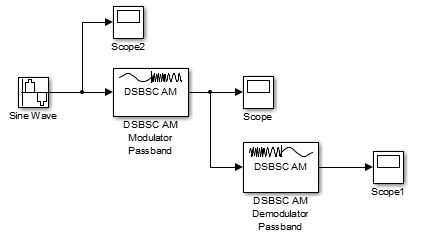
\includegraphics[width=6cm]{Sim_dsbsc0}
	\caption{Схема балансной модуляции/демодуляции}\label{fig.Sim_dsbsc0}
\end{figure}                                                                                                                                                                                                                                                                                                                                                                                                                                                                                                                                                                                                                                                                                                                                                                                                                                                                                                                                                                                                                                                                                                                                                                                                                                                                                                                                                                                                                                                                        

\begin{figure}[h]\centering
	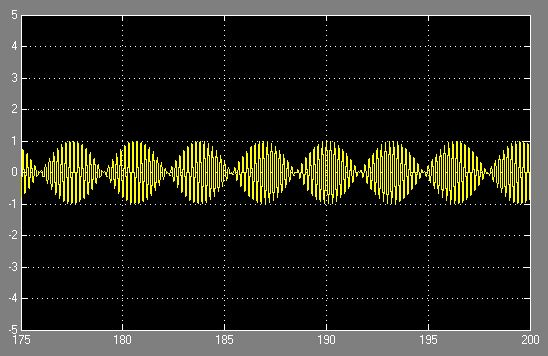
\includegraphics[width=8cm]{Sim_dsbsc2}
	\caption{БАМ-сигнал}\label{fig.Sim_dsbsc2}
\end{figure}                                                                                                                                                                                                                                                                                                                                                                                                                                                                                                                                                                                                                                                                                                                                                                                                                                                                                                                                                                                                                                                                                                                                                                                                                                                                                                                                                                                                                                                                        

\begin{figure}[h]\centering
	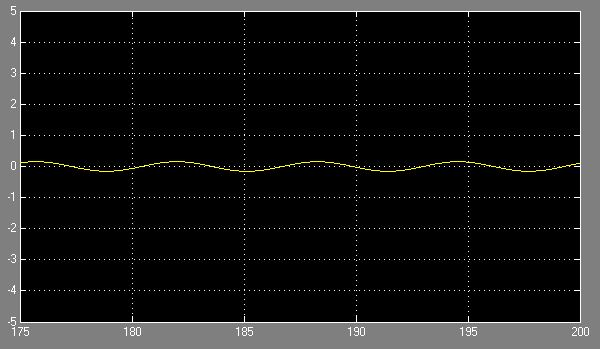
\includegraphics[width=8cm]{Sim_dsbsc3}
	\caption{Демодулированный БАМ-сигнал}\label{fig.Sim_dsbsc3}
\end{figure}                                                                                                                                                                                                                                                                                                                                                                                                                                                                                                                                                                                                                                                                                                                                                                                                                                                                                                                                                                                                                                                                                                                                                                                                                                                                                                                                                                                                                                                                        

\FloatBarrier

\subsection{Выводы}
В ходе выполнения лабораторной работы был сгенерирован однотоальный сигнал низкой частоты, выполнена АМ сигнала и получен спектр модулированного сигнала. Также была выполнена БАМ и однополосная АМ и получены их спектры. Произведено синхронное детектирование и получен исходный однополосный сигнал. Рассчитан КПД модуляции.

АМ применяется на сравнительно низких частотах (не выше коротких волн). Это обусловлено низким КПД использования энергии модулированных сигналов.

Ширина спектра АМ-сигнала с подавленной несущей, как  в случае с обычной АМ, в два раза больше, чем у модулирующего сигнала. Но при БАМ производится перемножение двух сигналов – модулирующего и несущего, при котором происходит подавление несущего колебания, соответственно, КПД модуляции становится равным 100\%. 

Двухполосная АМ с подавленной несущей имеет приемущества перед обычной АМ только в энергетическом плане - за счет устранения несущего колебанияю, ширина спектра при этом по-прежнему вдвое больше, чем у модулирующего сигнала. Однако спектры двух боковых полос АМ-сигнала являются зеркальным отражением друг друга, поэтому одну из боковых полос можно удалить.

Однополосный сигнал можно представить как сумму двух АМ-сигналов, несущие колебания которых имеют одну и ту же частоту, но сдвинуты по фазе относительно друг друга на $90^0$.

Синхронное детектирование является одним из способов демодуляции АМ-сигнала. Его суть состоит в умножении частоты сигнала на опорное колебание с несущей частотой. Результат умножения содержит два слагаемых: искомая амплитуда и АМ-сигнал с несущей частотой $2\omega_0$, который легко удаляется путем пропускания сигнала через ФНЧ. В нашем случае использовался фильтр Баттерворта.

\end{document}
